\documentclass[11pt]{article}
\usepackage{natbib}
\usepackage{float}
\usepackage[pdftex]{graphicx}     % could insert ``draft'' between []
\usepackage{amsmath}
\usepackage{amssymb}
\pagestyle{empty}
\setlength{\oddsidemargin}{0pt}
\setlength{\textwidth}{6.5in}
\setlength{\voffset}{0pt}
\setlength{\topmargin}{-0.75in}
\setlength{\textheight}{10.0in}
%%%%%%%%%%%
\newcommand\aj{\ref@jnl{AJ}}%
          % Astronomical Journal
\newcommand\actaa{\ref@jnl{Acta Astron.}}%
  % Acta Astronomica
\newcommand\araa{\ref@jnl{ARA\&A}}%
          % Annual Review of Astron and Astrophys
\newcommand\apj{\ref@jnl{ApJ}}%
          % Astrophysical Journal
\newcommand\apjl{\ref@jnl{ApJ}}%
          % Astrophysical Journal, Letters
\newcommand\apjs{\ref@jnl{ApJS}}%
          % Astrophysical Journal, Supplement
\newcommand\ao{\ref@jnl{Appl.~Opt.}}%
          % Applied Optics
\newcommand\apss{\ref@jnl{Ap\&SS}}%
          % Astrophysics and Space Science
\newcommand\aap{\ref@jnl{A\&A}}%
          % Astronomy and Astrophysics
\newcommand\aapr{\ref@jnl{A\&A~Rev.}}%
          % Astronomy and Astrophysics Reviews
\newcommand\aaps{\ref@jnl{A\&AS}}%
          % Astronomy and Astrophysics, Supplement
\newcommand\icarus{\ref@jnl{Icarus}}%
  % Icarus
\newcommand\mnras{\ref@jnl{MNRAS}}%
          % Monthly Notices of the RAS
\newcommand\prc{\ref@jnl{Phys.~Rev.~C}}%
          % Physical Review C
\newcommand\prd{\ref@jnl{Phys.~Rev.~D}}%
          % Physical Review D
\newcommand\pre{\ref@jnl{Phys.~Rev.~E}}%
          % Physical Review E
\newcommand\prl{\ref@jnl{Phys.~Rev.~Lett.}}%
          % Physical Review Letters
\newcommand\pasa{\ref@jnl{PASA}}%
  % Publications of the Astron. Soc. of Australia
\newcommand\pasp{\ref@jnl{PASP}}%
          % Publications of the ASP

\newcommand{\kvec}{{\bf k}}
\newcommand{\bvec}{{\bf b}}
\newcommand{\shat}{{\hat s}}
\newcommand{\kpr}{{k_\perp}}
\newcommand{\kvpr}{{\kvec_\perp}}
\newcommand{\kpl}{{k_\parallel}}
\newcommand{\AI}{{\langle\tilde A*\tilde I\rangle}}
\newcommand{\AItau}{{\AI(\tau)}}
\newcommand{\hMpci}{{h~{\rm Mpc}^{-1}}}
\newcommand{\inch}{$^{\prime\prime}$}
\newcommand{\foot}{$^{\prime}$}
\renewcommand{\deg}{^\circ}

\begin{document}
\title{Configuration of the HERA Element}
\author{Aaron Parsons \and David DeBoer}
\maketitle

\section{Introduction}

The design of the HERA element is driven by advances in our understanding of how
an interferometer's chromatic response interacts with foreground emission to
produce systematics in power spectral measurements of the 21cm reionization signal.

\section{Understanding Instrumental Chromaticity in the Context of the Wedge}

For this discussion, we average the three-dimensional power spectrum $P(\kvec)$ along a cylinder
of $k_x^2+k_y^2=\kpr^2$, where $\kvec\equiv(k_x,k_y,\kpl)$ is the three-dimensional wavevector,
$(k_x,k_y)$ are taken to be in the plane of the sky, and $\kpl$ is measured along the line-of-sight (spectral)
direction.
Recent work has shown that, for an interferometer whose
analog bandpass and beam chromaticity are sufficiently smooth, systematics arising from foreground emission
are isolated in the cylindrically averaged power spectrum $P(\kpr,\kpl)$ within
a wedge-shaped region \citep{2012ApJ...756..165P,2013ApJ...768L..36P,2014ApJ...788..106P,2015arXiv150206016A}:
% XXX add the whole list of wedge cites
\begin{align}
|\kpl| &\le \frac{Y}{X\nu}\kpr + YS\nonumber\\
&\le \frac{Y}{c}b + YS,
\label{eq:wedge_bound}
\end{align}
where $X,Y$ are cosmological scalars relating angular size and spectral frequency to comoving 
physical size, respectively, $\nu$ is spectral frequency, and $b=|\bvec|$ is the magnitude of the baseline vector for
antennas in an interferometric pair, which substitutes for $\kpr$ according to the
relation $\kvpr=X\nu\bvec/c$. As we will derive below, $S$ is an additional additive offset related to
the combined spectral smoothness of foregrounds and the antenna response.

As pointed out in \citet{2012ApJ...756..165P}, the factor of $b/c$ in the
second line of equation (\ref{eq:wedge_bound}) can be interpreted as the light-crossing time
or maximum geometric signal delay, $\tau_{b,max}$ associated with an interferometric baseline.  
Particularly for per-baseline
analyses such as those
employed on PAPER \citep{2014ApJ...788..106P,2015ApJ...801...51J,2015arXiv150205072M,2015arXiv150206016A},
{\it signal delay} turns out to be a 
powerful basis for understanding the chromatic effects of interferometric observations.
Signal delay arises as the Fourier dual to spectral frequency, according to the delay
transformation of a visibility,
\begin{equation}
\tilde V_\bvec(\tau)=\int{d\nu~V_\bvec(\nu) e^{2\pi i\tau\nu}}.
\end{equation}
The measurement equation defines the visibility as
\begin{equation}
V_\bvec(\nu)=\int{d\Omega~A(\shat,\nu)~I(\shat,\nu) e^{-2\pi i\frac{\bvec\cdot\shat}{c}\nu}},
\label{eq:meas_eq}
\end{equation}
where $A$ is the antenna response as a function of directon $\shat$ and $I$ is the sky intensity.
We define the geometric signal delay in direction $\shat$ as $\tau_{\bvec,\shat}\equiv\bvec\cdot\shat/c$
in order to re-express the delay-transformed visibility as
\begin{align}
\tilde V_\bvec(\tau)&=\int\!\!\int{d\nu~d\Omega~A(\shat,\nu)~I(\shat,\nu) e^{-2\pi i\nu(\tau_{\bvec,\shat}-\tau)}}\nonumber\\
&=\int{d\Omega~\tilde A(\shat,\tau)*\tilde I(\shat,\tau)*\delta_D(\tau_{\bvec,\shat}-\tau)},
\end{align}
where $\delta_D$ is the Dirac delta function, `$~\tilde{}~$' signifies Fourier transformation along
the frequency axis, and `$*$' denotes convolution.

Under the ``delay approximation" \citep{2012ApJ...756..165P},
signal delay $\tau$ can be interpreted as a reasonable approximation to $\kpl$, giving us the following relationship
between the delay-transformed visibility and the power spectrum:
\begin{equation}
\tilde V_\bvec^2(\tau)\approx\left(\frac{2k_B}{\lambda^2}\right)^2\frac{\Omega B}{X^2Y}\widehat P(\kvpr,\kpl),
\label{eq:v2_to_pk}
\end{equation}
where $k_B$ is Boltzmann's constant, $\lambda$ is spectral wavelength, $\Omega$ is the angular area of the power-squared
beam \citep{2014ApJ...788..106P}, and $B$ is the effective bandwidth over which the delay transformation is performed.

We can now revisit the bound on systematics arising from the interaction of foreground emission and
instrumental chromaticism given in equation (\ref{eq:wedge_bound}).  Let us assume for a moment that
$A$ and $I$ are perfectly flat functions of frequency, so that $\tilde A$ and $\tilde I$ are delta functions
centered at $\tau=0$.  In this case, the value of $\tilde V_\bvec(\tau)$ is determined by
the integral over $\tilde A(\shat,0)~\tilde I(\shat,0)$ in the sky directions that satisfy $\tau_{\bvec,\shat}=\tau$.
For a given baseline $\bvec=\kvpr/X\nu$, $\tau_{\bvec,\shat}$ is bounded by $\tau_{b,max}=b/c$, implying that
for the case we have outlined, $\tilde V_\bvec(\tau)$ must be zero outside of a region
$|\tau|\le b/c$.  Under the delay approximation, $\kpl\approx Y\tau$, so we can use equation
(\ref{eq:v2_to_pk}) and say that $P(\kpr,\kpl)$ must be zero outside of the region specified in 
equation (\ref{eq:wedge_bound}) for $S=0$.

The inclusion of $S$ in equation (\ref{eq:wedge_bound}) accounts for precisely the terms we neglected above:
the spectral structure in $A$ and $I$, or more precisely, the delay-domain width of 
\begin{equation}
\AItau\equiv\int{d\Omega~\tilde A(\shat,\tau)*\tilde I(\shat,\tau)},
\end{equation}
where $\langle\dots\rangle$ denotes the average over solid angle.
In order to determine $S$ quantitatively, however,
we must clarify what is the relevant width in delay-domain.  The purpose of equation (\ref{eq:wedge_bound}) is 
to illustrate
the boundary between the systematics-dominated and signal-dominated regimes.
As such, it makes the most sense to determine width by the interval in
delay domain outside of which $\AItau$ is below the expected level
of the 21cm reionization signal.  Spectrally smooth ($\tau\approx0$) foregrounds are approximately
four to five times brighter that the expected reionization signal \citep{unknown}, so a conservative definition of
$S$ requires
\begin{equation}
\frac{|\AItau|}{|\langle\tilde I\rangle(\tau=0)|}<10^{-6}.
\label{eq:def_S}
\end{equation}
In words, we define $S$ as the delay interval over which
$\AI$ falls off by -60 dB.  At this level, the contribution from antenna effects are well below the signal level in the region outside from where the foregrounds contaminate.  XXXWeak sentenceXXX

Given this framework, an obvious design goal for an interferometer aiming to 
measure the 21cm reionization signal is create antennas that can be close-packed to minimize $b$, and
which yield an antenna response that minimizes $S$.  However, as we will explore in more detail below, 
these goals must be balanced against cost.

% sky averaged 
\subsection{Inherent Chromaticity of Foregrounds}

Before we explore antenna design, however, it would be convenient to set an upper bound on the contribution of
$\tilde I$ in equation (\ref{eq:def_S}).   The result is strongly
dependent on windowing, however choosing a Blackman-Harris window and playing with power-law spectral indices of
-1 and -2, we find that a width for $\tilde I$ in range of 10 to 60 ns provides a reasonable bound.  This suggests diminishing returns associated with pushing instrumental chromaticity much lower than 10 to 60 ns.

Also, as we push antennas closer together, galactic synchrotron emission (our dominant foreground) gets
brighter as $C_\ell\propto\ell^{-3}$ \citep{unknown}.
Under the assumption that $\kpl$ is the dominant component of $\kvec$ (which
holds for the short baselines used in PAPER and HERA),
this implies that $|\AItau|^2$ must decrease more rapidly than $\tau^{-3}$ for a reduction in baseline length
to result in a reduction in foreground contamination at a given $\kpl$ scale.  Hence, the combined chromaticity
of the antenna beam and the galactic synchrotron foreground set an effective minimum baseline length, shorter
than which foreground systematics no longer decrease, and could even potientially extend further in $|\kpl|$.  
This departure from the
strictly linear relationship in equation (\ref{eq:wedge_bound}) (which we will call the ``ankle")
for the shortest baselines is a telltale sign
of the influence of diffuse synchrotron emission.

%%%XXX If get analytic derivation of foreground profile in delay working, relate to that here.
Figure 3 in \citet{2013ApJ...768L..36P}
shows evidence of the departure equation (\ref{eq:wedge_bound}) described above for baselines shorter than
$\lesssim10$ wavelengths.  Although this empirical result includes a contribution from the PAPER antenna beam,
the constant additive term that $\tilde A$ contributes (which is baseline dependent)
to the wedge boundary does not change the position of the ankle.  Also worth noting is that, although an ankle
appears around $\sim9$ wavelengths, the extent of the wedge in $\kpl$ continues to decrease slowly toward 
even shorter baselines.  This implies that, while there are diminishing returns in foreground systematics for using
baseline shorter than $\sim18$ m (9 wavelengths at 150 MHz), there does not appear to be a strong penalty 
for doing so either.

\subsection{Antenna Chromaticity}

So far, we have largely ignored the contribution of the antenna term in $\AItau$.  We now have
a handle on the chromaticism introduced by the baseline term in equation (\ref{eq:meas_eq}) and 
an indication of when shorter baselines stop linearly reducing the occupancy of
foreground systematics in $|\kpl|$.  As we argued above, $b\lesssim20$ m is an approximate threshold
for when the chromaticity of the baseline term is no longer dominant.  This suggests that
foreground systematics are unlikely to drop below a width in delay domain corresponding to 
$b/c\sim60$ ns ($|\kpl|\sim0.03\hMpci$ at 150 MHz).

Therefore, a reasonable specification 
for an interferometer targeting 21cm power spectrum measurements and working outside
the wedge to avoid foregrounds might be to equally partition a chromaticity budget (i.e. delay-domain
width) between the baseline term $\delta_D(\tau_{\bvec,\shat}-\tau)$, 
the inherent foreground term $\tilde I(\shat,\tau)$, and the antenna term $\tilde A(\shat,\tau)$.
As described in equation (\ref{eq:def_S}), the relevant delay domain width 
is measured at the -60 dB point.  Therefore, the specification we set for the chromaticity
of the antenna is
\begin{equation}
\frac{|\langle\tilde A\rangle(\shat,\tau=60~{\rm ns})|}{|\tilde \langle A\rangle(\shat,\tau=0~{\rm ns})|}<10^{-6}.
\label{eq:A_req}
\end{equation}
Here, we have separated the antenna and sky terms in $\AItau$ in order to set a specification for
the antenna term alone.

Under this specification, we assume the final chromaticity (wedge width) to be the sum of the
individual widths of the $\tilde A$, $\tilde I$, and $\delta_D(\tau_{\bvec,\shat}-\tau)$ terms,
for a total of 180 ns ($|\kpl|=0.9\hMpci$ at 150 MHz).

% XXX below here treating as memo, not paper
\section{HERA Element Design}

As shown above, the delay-spectrum analysis technique employed for HERA requires that foreground
systematics be tightly bounded within a wedge-shaped region in $(\kpr,\kpl)$ space,
such that contamination outside of this region falls
below the expected level of the 21cm reionization signal.
The supplied value from the analysis team is that reflections must be reduced
by at least -60 dB at 60 ns.  Another formulation is VSWR $<$ 1.002 integrated over fluctuation scales of $\Delta\nu\leq17$ MHz.

Assuming that HERA elements will have to deliver substantially more collecting area per feed
than the current PAPER design, we adopted a parametrizable design based on a parabolic dish
with a feed suspended over it.
Thus, the optics of the HERA dish is set by three factors:  
\begin{enumerate}
\item meeting the chromaticity specification of -60 dB at 60 ns,  (Eq. \ref{eq:A_req})
\item minimizing the impact of baseline-coupling systematics, and 
\item minimizing cost for a fixed sensitivity
\end{enumerate}
The relevant parameters are the diameter ($D$), the focal length ($f$) and the overall sensitivity (essentially, $N$, the total number of elements).  Antenna chromaticity is largely determined by the focal length (at least as a design parameter), and the discussion will focus on that.

 \subsection{Focal Length}
Optimizing the focal length comes down to simultaneously optimizing the $f/D$ for system performance and $f$ for delay performance (chromaticity).  We discuss both of these aspects below.

\subsubsection{Efficiency}
Assuming a feed based on the PAPER design for a backplane without flaps,
we computed a series of analytical models at 150 MHz versus diameter over a 3.4--4.6 m range in focal height
for an ideal parabolic dish.  These models were used to determine the total efficiency of
feed/reflector system, with efficiency $\eta$ computed as the effective collecting area
relative to the total geometric collecting area of a circular aperture of the
indicated diameter.
As shown in Figure \ref{fig:efficiency},
model efficiencies peak at $\eta\approx0.73$ for focal ratios of $f/D\approx0.32$ (the solid lines with the x-axis divided by 10), largely
independent of the absolute scale of diameter.

\begin{figure}[h]
\centering
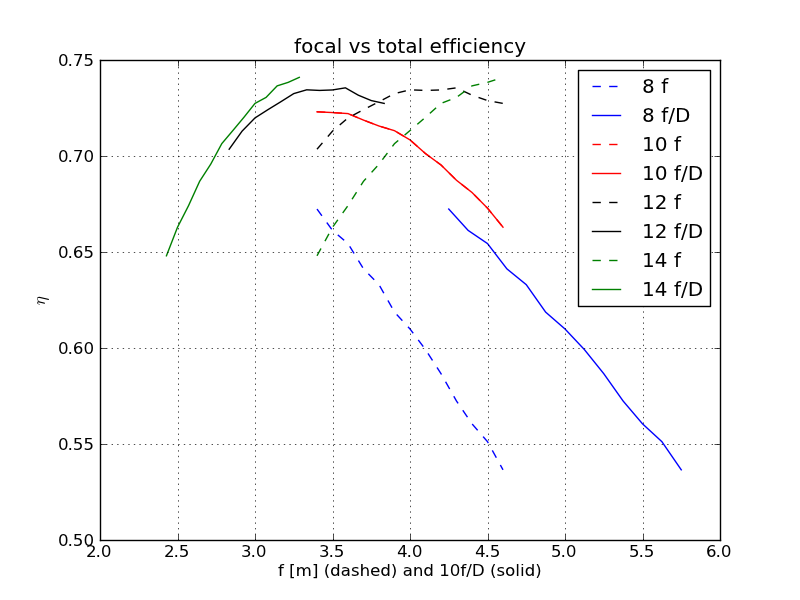
\includegraphics[width=0.8\textwidth]{heraDishfDplot.png}
\caption{The model efficiency of a PAPER feed suspended over an ideal parabolic dish.  
The dashed curves indicate the efficiencies over a 3.4--4.6 m range in focal height $f$
for the dish diameters $D$ indicated in the legend.  The solid curves extrapolate the
model efficiencies of the corresponding dashed curves to a $D=10$ m dish (note
the red dashed and solid curves are identical). The approximate agreement of the
solid curves indicates that to first order, efficiency is a function
of the focal ratio $f/D$. The absolute scaling of $\eta$ with $D$ appears as a second-order (few percent) increase in efficiency.  Hence, peak efficiencies of order $\eta\approx0.73$ are expected for
focal ratios of $f/D\approx0.32$.}
\label{fig:efficiency}
\end{figure}

\subsubsection{Chromatic Effects}
The dominant source of chromaticism within the antenna can be identified with internal signal 
reflections, with delays set largely by the focal length.  Diffraction around dish edges and the evolving 
response of the feed also introduce chromaticism, but the scale of these frequency-dependent effects 
are expected to be significantly broader than the specified 17 MHz scale.  In order to be problematic, 
signal reflections originating at the feed must re-enter the feed after a time delay of 60 ns before they 
are attenuated by 60 dB.Taking a geometric interpretation for an ideal paraboloid, off-axis emission 
from the feed is reflected out to the sky without re-entering the feed.Therefore, the dominant source of 
reflections is expected to arise between the feed and vertex.If reflections between the feed and vertex 
are dominant, as noted above, the most important determinant of the timescale of reflections will be the 
feed height above the vertex.  

Here, we adopt the focal ratio of $f/D=0.32$ derived in the previous section in
the context of maximizing efficiency.  In doing so, we reduce the parametrization of our parabolic
dish to a single degree of freedom: the diameter $D$ (or, equivalently $f$).  We may then explore how the timescale and amplitude of reflections between the feed and the vertex of the paraboloid scale with $D$.

Although not properly adequate, we will use a geometric (far-field) model as a tool for determining coarse scaling relationships.  Geometrically, waves arriving at the feed from the sky absorbed and reflected in accordance with the impedance match between free space and the feed/balun system.  The reflected wave is essentially re-emitted from the feed into the dish, and bulk of it is reflected back to the
sky.  However, as discussed previously, emission toward the the vertex of the parabola may be reflected
back toward the feed, whereupon the absorption/reflection process repeats with an attenuated amplitude.

\begin{figure}[h]
\centering
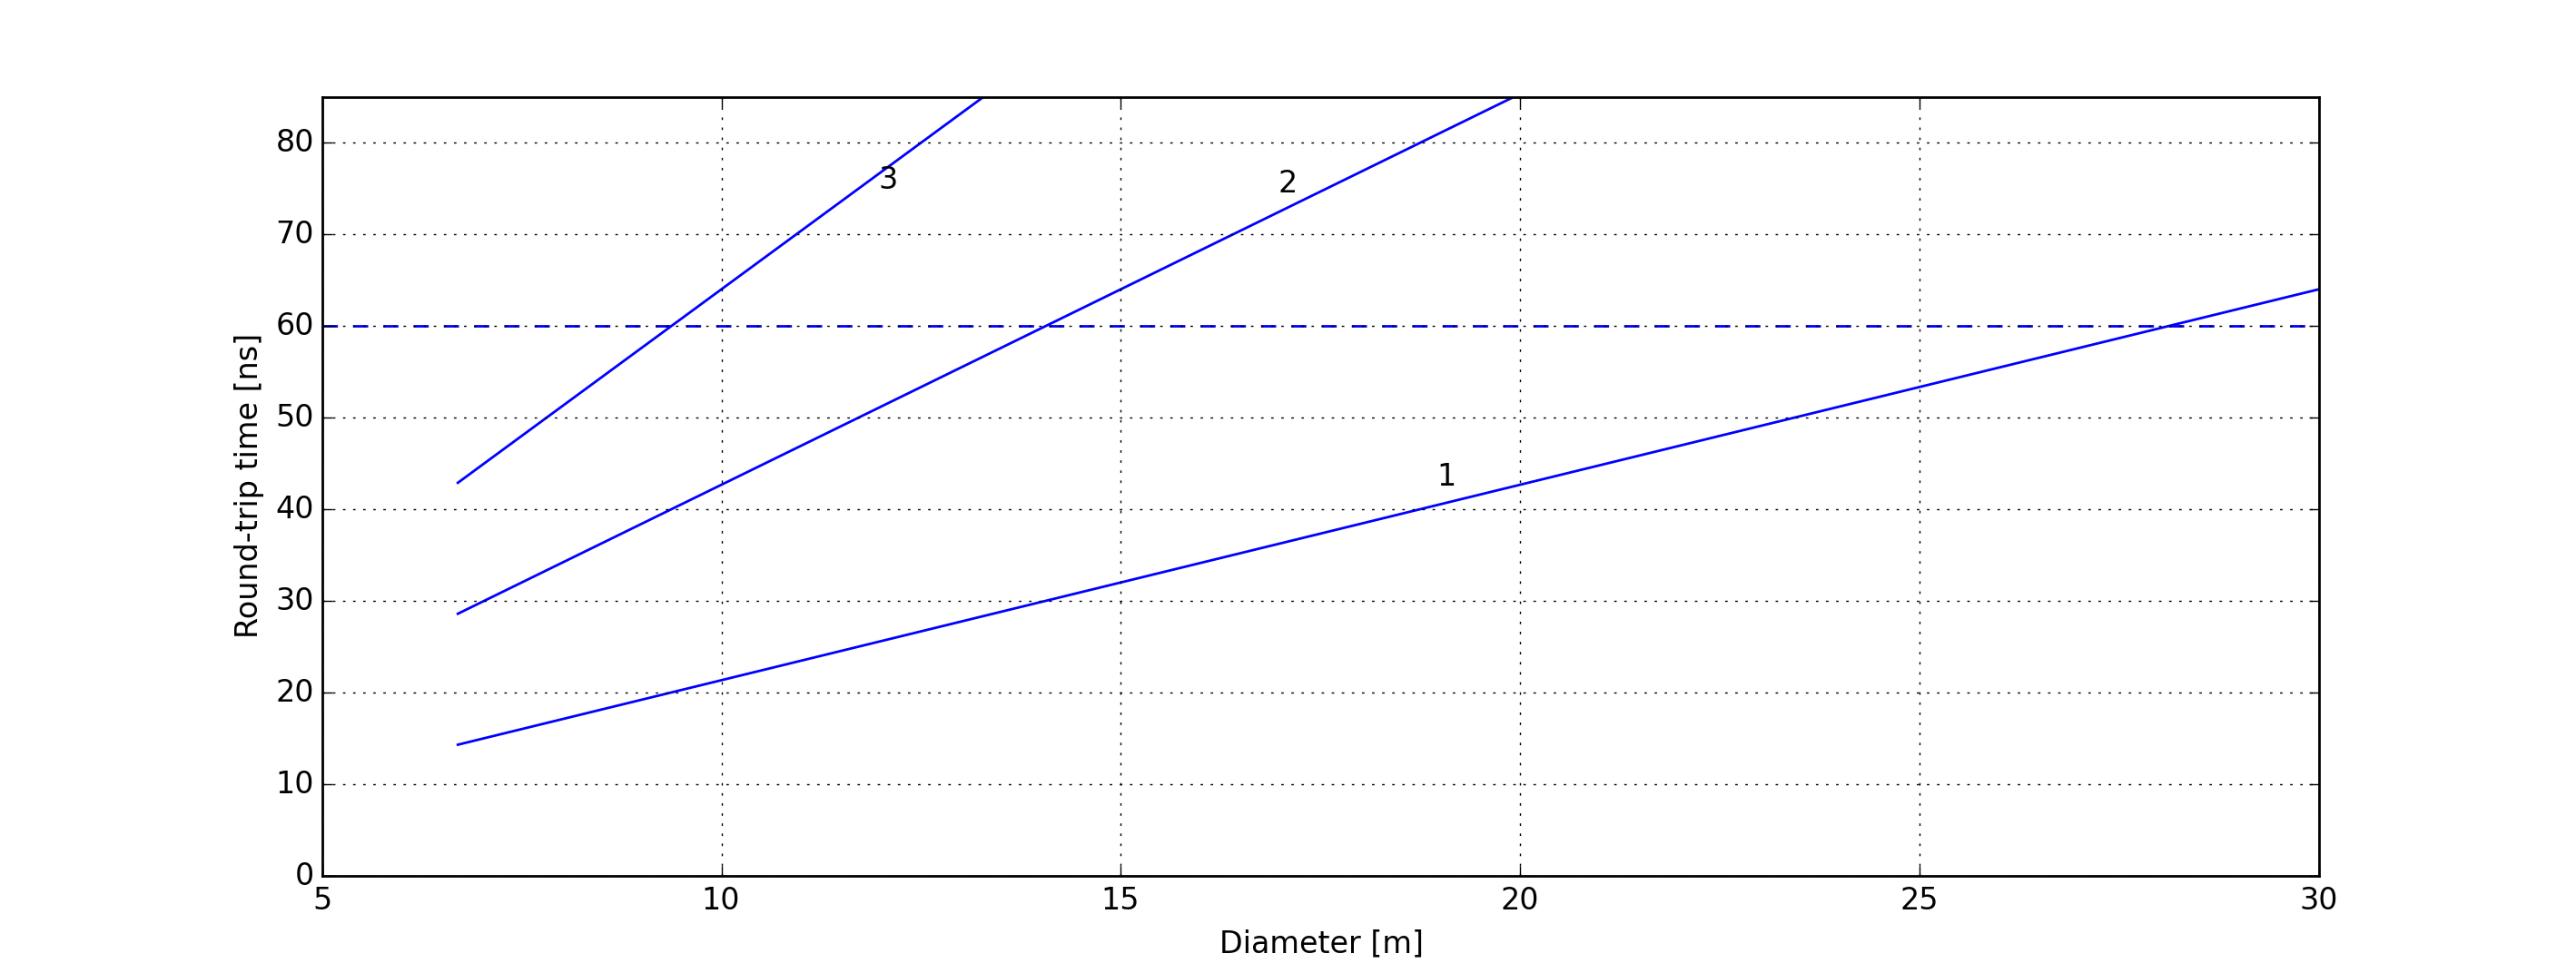
\includegraphics[width=1.0\textwidth]{roundtrip.png}
\caption{Round-trip propagation times between feed and vertex for $f/D=0.32$, 
shown for 1, 2, and 3 reflections.  The 60-ns timescale appearing in the specification
is indicated with a dashed line.}
\label{fig:roundtrip}
\end{figure}

We begin by computing the round-trip light-propagation times between the vertex and feed.  Figure
\ref{fig:roundtrip} shows the resulting signal delay for reflections spanning 1, 2 and
3 round trips.  To interpret the results, let us explore different cases.
If we assume that after two reflections, the reflected signal has been attenuated
below the -60 dB threshold in the specification, then the first reflection (which is above the
threshold) must have a timescale shorter than 60 ns.  Following the curve for 1 round-trip
reflection, we see that a 28-m dish (with a focal height of $\sim9$ m) is the maximum size
that would meet the specification.  If, on the other hand, a 60 dB attenuation is only achieved on the
third reflection, then the curve for 2 round trips suggests a maximum diameter of 14 m.  Similarly,
requiring the attenuation associated with one more reflection moves the maximum diameter down
to 9.4 m.

\begin{figure}[h]
\centering
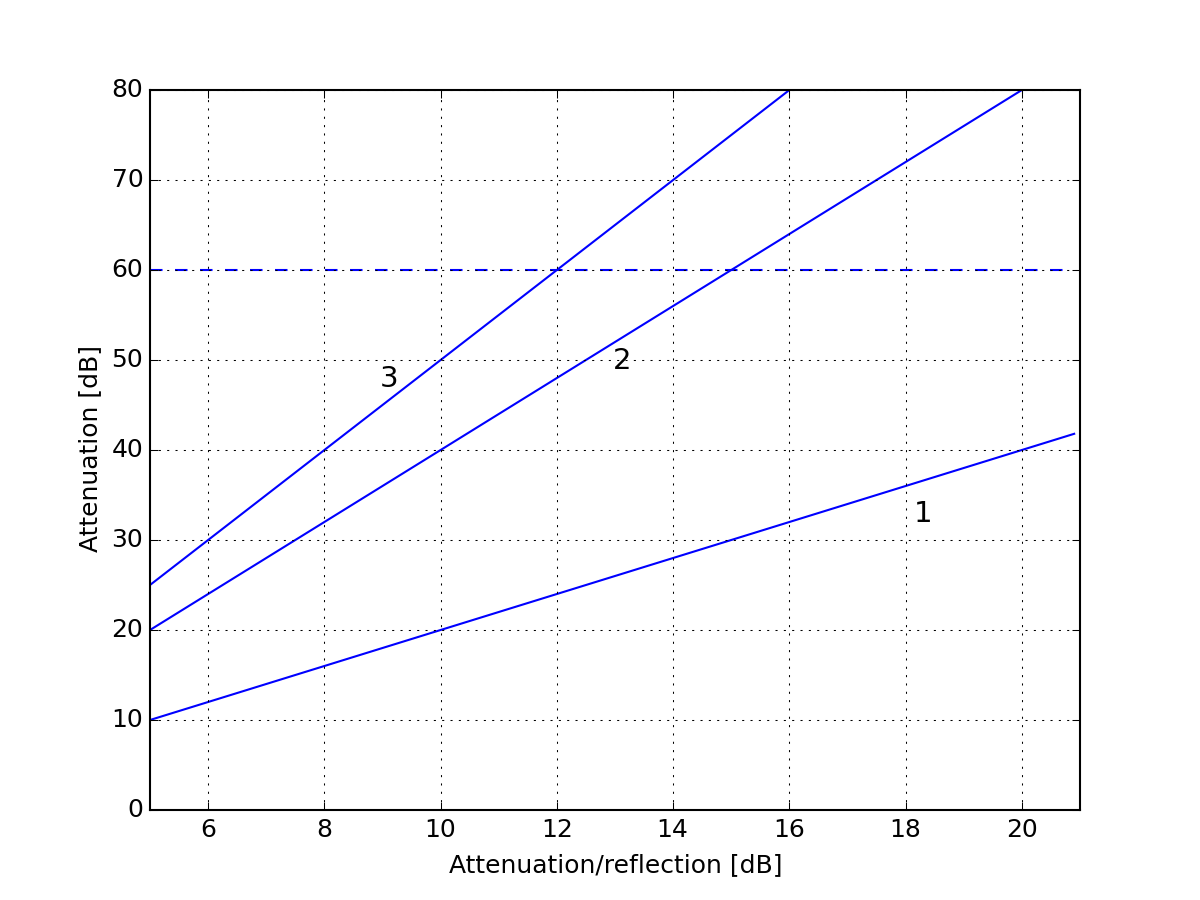
\includegraphics[width=1.0\textwidth]{bounces.png}
\caption{Overall attenuation for 1, 2 and 3 trips.
} \label{fig:bounces}
\end{figure}

Finally, we may ask, given the number of reflections that fall inside of 60 ns,
what is the attenuation per reflection $\Gamma$ that puts the signal level below
-60 dB after 60 ns?  Here, $\Gamma$ includes all loss factors, including the 
reflection coefficient associated with the impedance match of the feed,
path loss, etc.  Illustrated in Figure \ref{fig:bounces} is the total attenuation 
of a signal arriving at timescales $<$60 ns,
given as a function of $\Gamma$ for the indicated number of reflections falling
inside 60 ns.

Combining the results in Figures \ref{fig:roundtrip} and \ref{fig:bounces},
we can see that dishes with $D<9.4$ m must have $\Gamma<-12$ dB, dishes
where $9.4~{\rm m}<D<14~{\rm m}$ require $\Gamma<-15$ dB, and those with
diameters $14~{\rm m}<D<28$ m need $\Gamma<-30$ dB.

It is worth noting that imperfect impedance matches in the feed as a function
of frequency generally place the reflection coefficient of the feed itself
in the range of -5 to -15 dB. We must rely on directing reflected
waves away from the feed to achieve the total attenuation per reflection
that is required.  Geometrically, we can estimate that for a parabolic reflector that
reflects emission from the feed straight upward, a wave must intersect the paraboloid
at a distance of half a wavelength off axis to avoid
passing close enough to the feed to be re-absorbed.  Assuming $\lambda=2$ m, this angle is 
\begin{equation}
\phi\approx\tan^{-1}\frac{1}{f}.
\end{equation}
For a 14-m dish with a focal ratio of $f/D=0.32$ ($f\approx4.5$ m), $\alpha\approx13^\circ$.
This gives a solid angle of 0.15 sr into which the feed must emit in order to receive the reflection.
We can calculate the power emitted into this region numerically given a model of the feed response,
but coarsely, for a feed emitting uniformly into $2\pi$ sr, the power emitted into this region
represents -16 dB of the total reflected power.  

Thus, it seems likely that $\Gamma\sim-15$ dB is achievable, while $\Gamma\sim-30$ dB
would require very careful tuning of the feed and dish, if possible at all.

INCLUDE PLOT OF RELECTOMETRY TESTS

\section{Systematics}

As described above, minimizing internal reflections that introduce signal delays is
the primary design requirement of the HERA dish.  A secondary consideration is the
reduction of cross-coupling between the feeds of adjacent dishes.  Since the focus of
the parabolic dish lies above the rim, feeds potentially have a direct line of sight to
one another.  Noise and signal reflections emanating from one feed and coupling into another
can introduce spurious correlations that show up, to first order, as a static (zero fringe rate) additive
phase term with significant spectral structure.  

Although current PAPER analysis removes such static correlations via fringe-rate filtering, this
approach limits observing to regions away from the celestial poles, and significantly reduces the number
of independent sky samples obtained with a given baseline.  Although this approach may remain an
imporant tool for dealing with feed cross-coupling, it would be nice to limit its necessity.
One obvious way to do this is to shield feeds from one another.

To achieve this, the HERA dish design incorporates mesh screens at the boundaries of dishes that rise high
enough to shield feeds from one another.  In the limit of geometric optics, these screens perfectly isolate
feeds from one another, but risk introducing a new internal reflection pathway.  To avoid reflecting signals back into the feed,
screens may be tilted such that a ray originating from the feed and arriving at the screen are
reflected upward far enough that they miss the feed by a wavelength.
For a dish with a radius of $\sim7$ m and an observing wavelength of $\sim$2 m, this requires a tilt angle $\alpha$
given by $\tan\alpha=1/7$.  Thus, in the geometric limit, shielding screens must be approximately 8 degrees off of vertical.

In practice, the geometric optical limit is not met, and the above specification can only be a coarse rule of thumb.
Most notably, the top edge of the screen will introduce diffraction that degrades feed-feed isolation.  Scalloping
or rolling the edges of screens may help reduce diffraction, but these ideas will need to be tested in the field to
show their efficacy.

Pending field testing, HERA dishes are designed to include screens that rise $\sim2$ m from the rim ($\sim$0.75 m above the 
feeds), supported
by the same large wooden poles that are used to suspend the feed.  The bottom of these screens are held at a distance of
30 cm inward relative to the top, for a tilt of 8.5 degrees from vertical.

\section{Sensitivity}
The equation for sensitivity has been described in previous works \cite{unknown} and depends on many parameters
related to the instrumentation, the configuration, the location, the observing strategy, etc.  A useful form for 
the proposed compact configuration is Eq 27 in \citep{2012ApJ...753...81P} and reproduced here:
\begin{equation}
\centering
\label{eq:sensitivity}
\begin{split}
\Delta^2_N(k) \approx 60 \left[\frac{k}{0.1h\text{Mpc}^{-1}}\right]^\frac{5}{2}
                                         \left[\frac{6 \text{MHz}}{B}\right]^\frac{1}{2}
                                         \left[\frac{1}{\Delta\ln k}\right]^\frac{1}{2} \\
                        \times       \left[\frac{\Omega}{0.76\text{sr}}\right]
                                         \left[\frac{T_\text{sys}}{500 \text{K}}\right]^2
                                         \left[\frac{6 \text{hrs}}{t_\text{per\_day}}\right]^\frac{1}{2} \\
                        \times       \left[\frac{120\text{days}}{t_{\text{cam}}}\right]
                                         \left[\frac{32}{N_a}\right]
                                         \left[\frac{\text{10}^4f_o}{f}\right]  \text{mK}^2
\end{split}
\end{equation}
where $k$ is the magnitude of the $k$-mode, $B$ is the bandwidth, $\Delta\ln k$ is the log
of the binsize, $\Omega$ is the field-of-view, $T_{\text{sys}}$ is the system temperature, 
${t_\text{per\_day}}$ is the number of hours observed per day, $t_{\text{cam}}$ is the number of days
observed, $N_a$ is the number of antennas, and $f_o/f$ is the configuration metric for a 
redundant array as defined in \citep{2012ApJ...753...81P}.

Note that $\Delta^2_N(k)$ is the standard radiometric sensitivity equation, scaled by
the volume in $k$-space, normalized by the power spectrum Fourier coefficient, and
reduced by the number of independent samples in a given $k$-mode bin, which may have
both coherent and incoherent application.

Pulling out terms relating to diameter ($D_a$) and number, we can write Eq. \ref{eq:sensitivity} as
\begin{equation}
\label{eq:reducedSensitivity}
\Delta^2_N(k) \propto \frac{\Omega (f_o/f)}{N_a\sqrt{t_\text{per\_day}}} \propto \frac{(1/D_a^2)(1/\sqrt{N_a})}{N_a\sqrt{D_a}}
= D_a^{-\frac{5}{2}}N_a^{-\frac{3}{2}}
\end{equation}
where the dependencies on diameter and number have been substituted in, noting that the expressions for $f_o/f$ and 
$t_\text{per\_day}$were derived in Parsons et al where the baselines for the close-packed array are multiples of the diameter.

Letting the reduced sensitivity be $C = D_a^{-\frac{5}{2}}N_a^{-\frac{3}{2}}$ and scaling for canonical values of $D_a = 14$ m, $N_a = 331$ m, the needed number of antennas as a function of diameter (shown in Fig \ref{fig:Nsens}) is
\begin{equation}
\label{eq:Nmetric}
N_a = 26918 D_a^{-\frac{5}{3}}
\end{equation}

\begin{figure}[h]
\centering
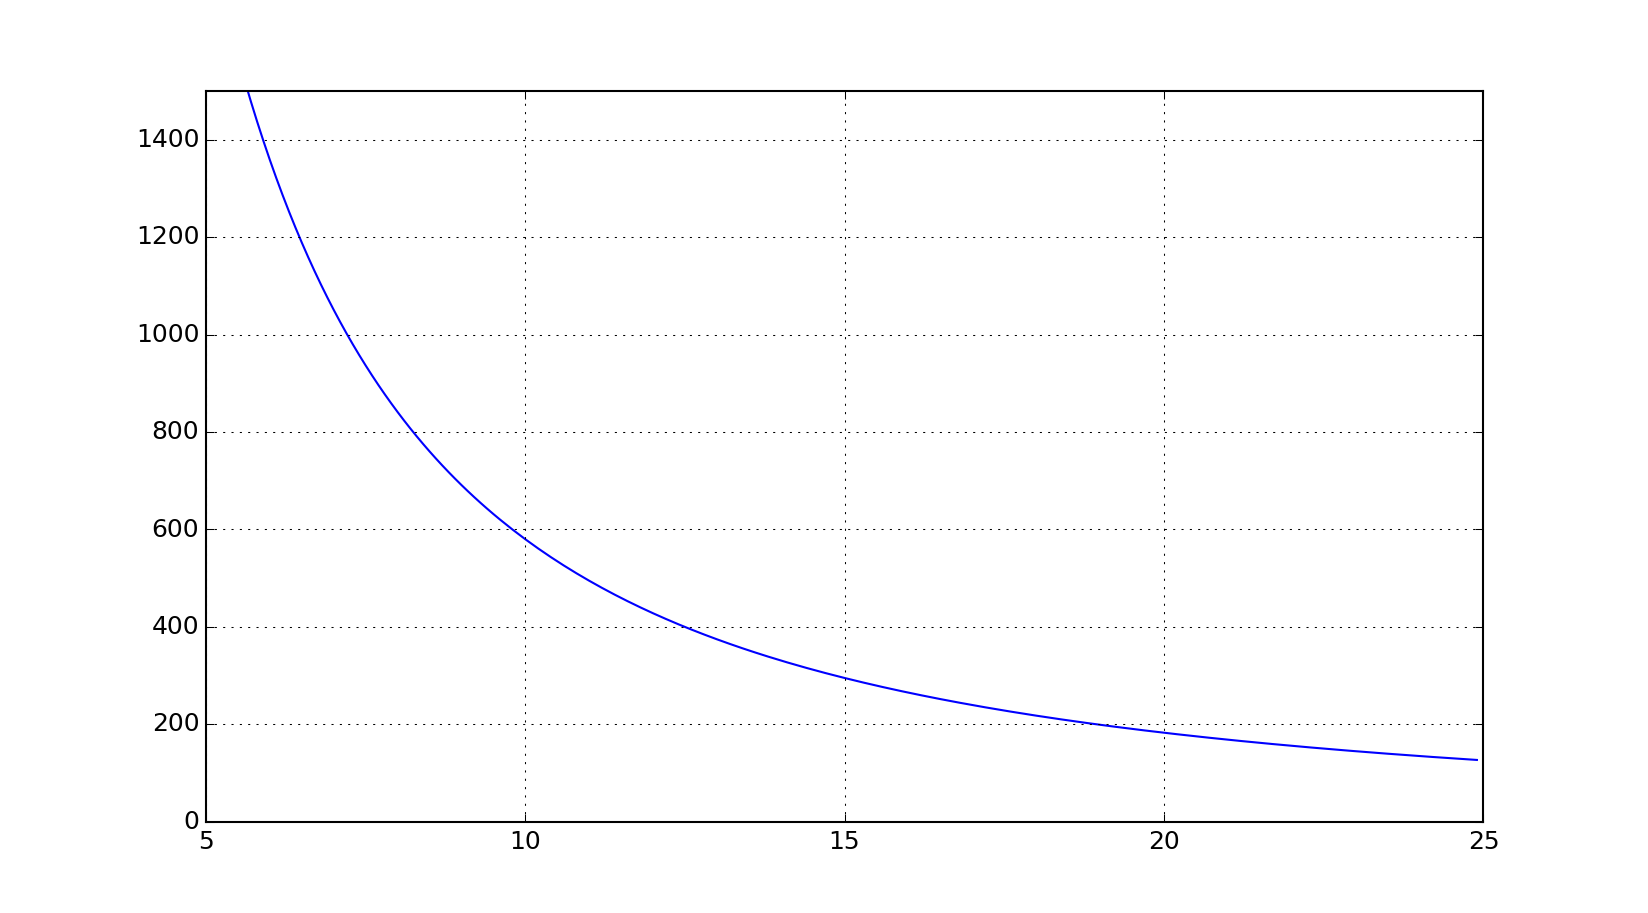
\includegraphics[width=0.8\textwidth]{Nsens.png}
\caption{Number of antennas at fixed sensitivity with reference of 331 14-m antennas}
\label{fig:Nsens}
\end{figure}

The sensitivity specification is to maximize performance per cost, which determines the element 
diameter ($D_a$) and the number of elements ($N_a$) subject to the constraints above.  One therefore 
needs a model of cost and performance as a function of $D_a$ and $N_a$.  Given a fairly mature element
and system design, a bottoms-up costing appropriate for element diameters from about 6-m to 30-m 
has been done for hex-numbers corresponding to element counts from 91 to 1141.  The costs here
are only those associated with delivering the array to that scope on-site, so excluding development and
science.  The results are shown in Fig. \ref{fig:normcost}.  At diameters greater than about 12-m the cost function
is relatively flat.

\begin{figure}[h]
\centering
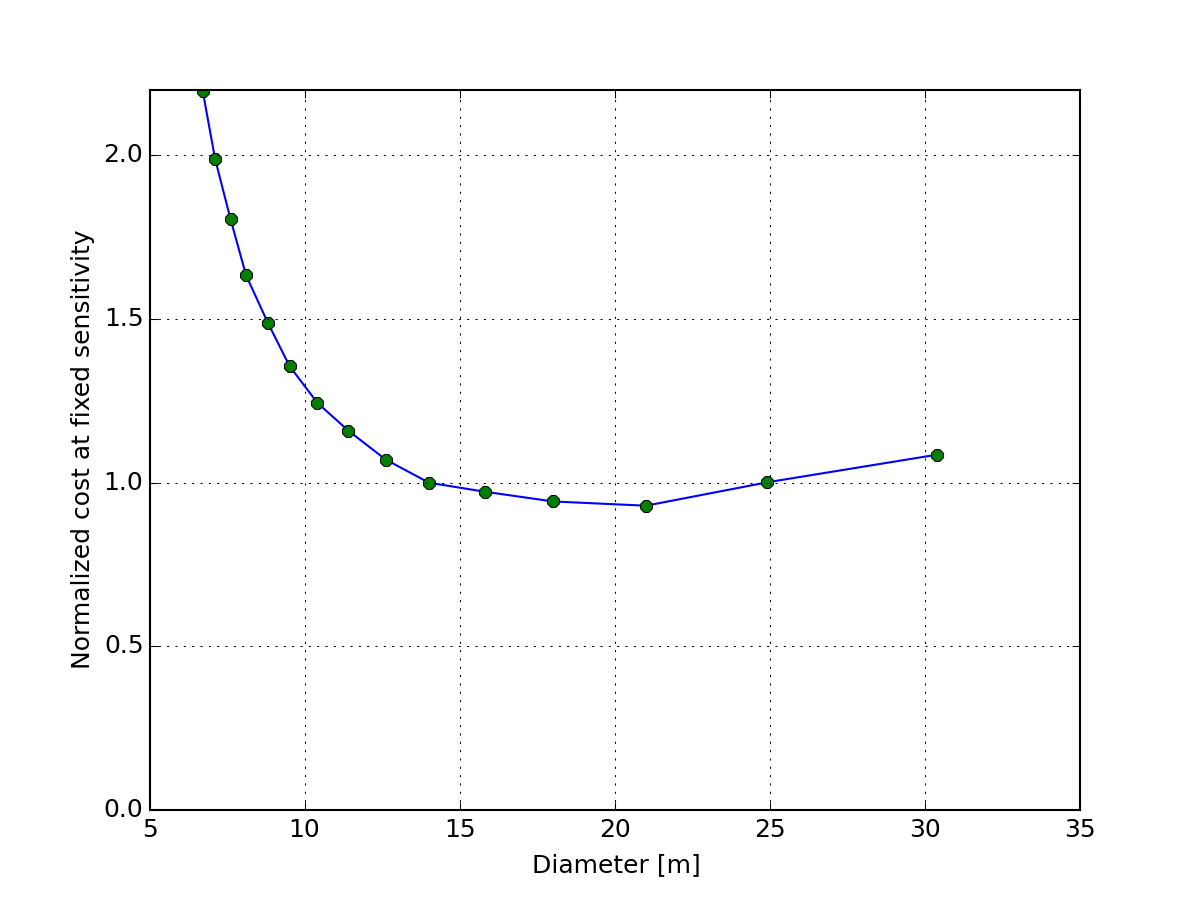
\includegraphics[width=0.8\textwidth]{normcostfunc.png}
\caption{Normalized cost at fixed sensitivity with reference of 331 14-m antennas}
\label{fig:normcost}
\end{figure}

\bibliographystyle{plainnat}
\bibliography{mybibdesk.bib}
\end{document}
